%!TEX root = ../../main.tex

\chapter{Vorstellung der MVC-Architektur}
\label{chap:vorstellung}

Das Model-View-Controller (MVC) Pattern ist ein bewährtes Software-Architekturmuster, dass die Strukturierung von Anwendungen in drei Hauptkomponenten vorsieht: Model, View und Controller. Diese Trennung der Verantwortlichkeiten erleichtert die Wartung und Erweiterung der Anwendung und fördert die Wiederverwendbarkeit und Testbarkeit der einzelnen Komponenten. MVC wurde ursprünglich für die Benutzeroberflächenentwicklung in Smalltalk (Programmiersprache) entwickelt und hat sich seitdem als Standard für die Strukturierung von Webanwendungen etabliert.

Das MVC-Pattern ist besonders nützlich in komplexen Anwendungen, bei denen eine klare Trennung zwischen Daten, Benutzeroberfläche und Steuerungslogik erforderlich ist. Es ermöglicht Entwicklern, sich auf spezifische Aspekte der Anwendung zu konzentrieren, ohne sich um die anderen Teile kümmern zu müssen. Dies führt zu einer besseren Organisation des Codes und erleichtert die Zusammenarbeit in Teams.


\section{Eigenschaften}

Das MVC-Pattern teilt eine Anwendung in drei Hauptkomponenten, die jeweils spezifische Aufgaben und Verantwortlichkeiten haben. Diese Hauptkomponenten werden im folgenden genauer erklärt:
\begin{itemize}

\item Model: Diese Komponente repräsentiert die Daten und die Geschäftslogik der Anwendung. Sie ist verantwortlich für das Abrufen, Speichern und Verarbeiten von Daten. Das Model benachrichtigt die View über Änderungen, sodass die Benutzeroberfläche aktualisiert werden kann. Das Model enthält die Kernfunktionalität der Anwendung und ist unabhängig von der Benutzeroberfläche.

\item View: Die View-Komponente stellt die Benutzeroberfläche dar. Sie zeigt die Daten des Models an und sendet Benutzereingaben an den Controller weiter. Die View ist für die Darstellung der Daten zuständig und reagiert auf Änderungen im Model. Sie ist passiv und kennt die Geschäftslogik nicht; sie zeigt nur die Daten an, die ihr vom Model bereitgestellt werden.

\item Controller: Der Controller verarbeitet die Benutzereingaben, interagiert mit dem Model und aktualisiert die View entsprechend. Er fungiert als Vermittler zwischen Model und View und steuert den Datenfluss zwischen diesen Komponenten. Der Controller interpretiert die Eingaben des Benutzers und ruft die entsprechenden Methoden im Model auf, um die Daten zu ändern. Anschließend aktualisiert er die View, um die neuen Daten anzuzeigen.

\end{itemize}
Diese Struktur ermöglicht eine klare Trennung der Verantwortlichkeiten, was die Wartbarkeit und Erweiterbarkeit der Anwendung erleichtert. Entwickler können Änderungen an einer Komponente vornehmen, ohne die anderen Komponenten zu beeinflussen. Dies ist besonders nützlich in großen Projekten, bei denen mehrere Entwickler gleichzeitig an verschiedenen Teilen der Anwendung arbeiten.

\section{Grafische Darstellung}

Ein Klassendiagramm für das MVC-Pattern könnte wie folgt aussehen. Es zeigt die Beziehungen und Interaktionen zwischen Model, View und Controller.

\begin{figure}[h]
\centering
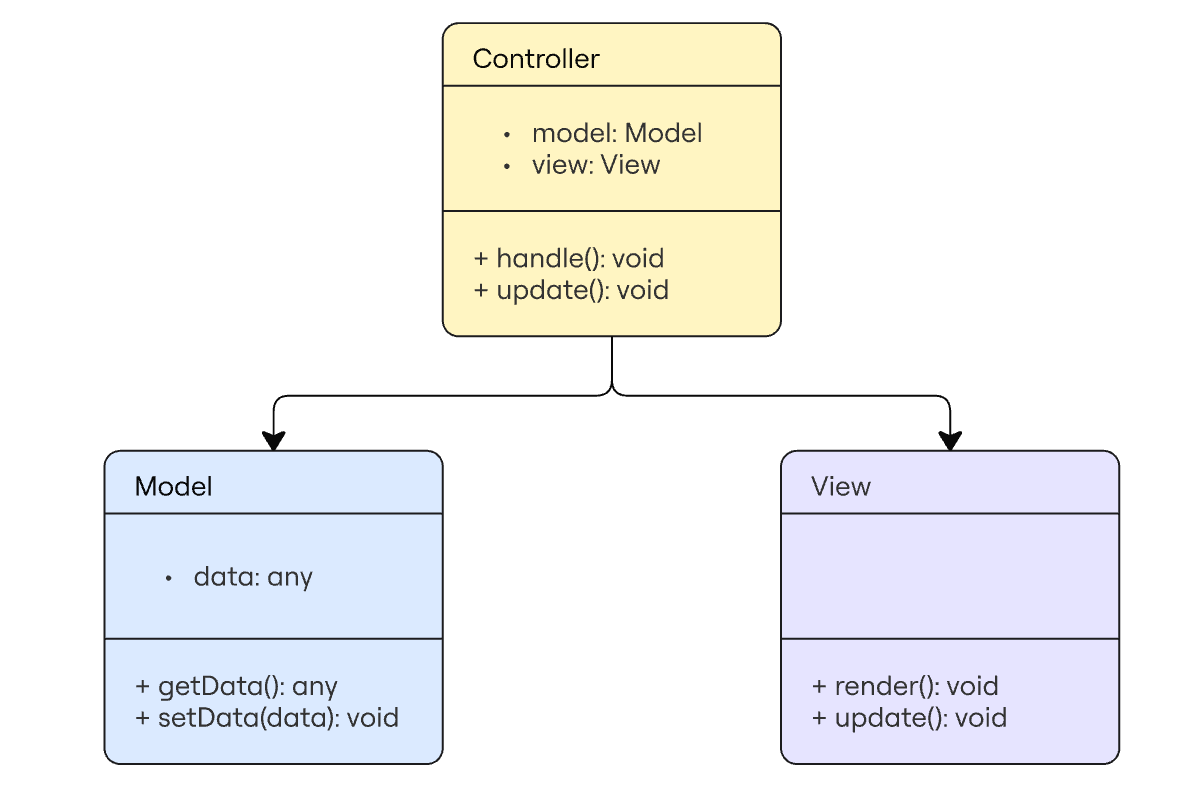
\includegraphics[height=.6\textwidth]{Klassendiagramm.png}
\caption{Das Logo der Musterfirma\footnotemark}
\end{figure}

In diesem Klassendiagramm sehen wir die folgenden drei Komponenten:

\begin{itemize}
\item Der Controller enthält Referenzen auf das Model und die View und hat Methoden zum Verarbeiten von Eingaben und Aktualisieren der View. Er ist das Bindeglied zwischen Model und View und sorgt dafür, dass die Benutzerinteraktionen korrekt verarbeitet werden.

\item Das Model enthält die Daten und Methoden zur Datenmanipulation. Es stellt die Geschäftslogik der Anwendung dar und ist unabhängig von der Benutzeroberfläche.

\item Die View enthält Methoden zur Darstellung der Daten und zur Aktualisierung der Benutzeroberfläche. Sie zeigt die Daten an, die vom Model bereitgestellt werden, und reagiert auf Änderungen im Model.
\end{itemize}

Die Interaktionen zwischen den Komponenten sind wie folgt:

\begin{enumerate}
\item Der Benutzer interagiert mit der View (z.B. durch Klicken auf einen Button).

\item Die View sendet die Benutzereingabe an den Controller.

\item Der Controller verarbeitet die Eingabe und aktualisiert das Model.

\item Das Model benachrichtigt die View über die Änderungen.

\item Die View rendert die aktualisierten Daten.
\end{enumerate}

Diese Abfolge zeigt, wie die Komponenten zusammenarbeiten, um Benutzereingaben zu verarbeiten und die Benutzeroberfläche zu aktualisieren. Die klare Trennung der Verantwortlichkeiten erleichtert die Wartung und Erweiterung der Anwendung und fördert die Wiederverwendbarkeit und Testbarkeit der einzelnen Komponenten.